\section{People in the place}\label{people-in-the-place}

\subsection{Routes and joined motion}\label{routes-and-joined-motion}

Each walker is given spots to pass through and the length of its film. Its route is the shortest way through those spots over the check's own walkers' floor, with doors open as passages and a stair flight as a run of spans one riser apart, its corners kept by line of sight and rounded over 0.6 m, so a route never leaves floor the check has judged. A walker that must fill its film walks on around its spots until it does. The route is then timed at 1.0 m/s on the flat and one tread per step on a flight, eased from standing at the start and back to standing at the end, and cut into pieces of at most 7 s at every start and end of a flight. Each piece is generated by Kimodo \citep{rempe2026kimodo} in its own canonical frame from the dense path and heading of its stretch, as a flat walk or as a climb with each foot asked onto its tread. Every piece after the first is constrained by full-body keyframes on its first four frames to the pose in which the previous piece stood there, so that position and velocity match across the join. The pieces are joined back in the scene's frame by blending over those shared frames, with the standing foot held on its spot. The travel therefore comes from the clips themselves; a clip is never slid, stretched or looped along a line. Each walker is measured against fixed limits: foot skate per stance of at most 2 cm, the hips within 10 cm of the route, and the body clear of every upright solid between knee and head.

\subsection{Sim bodies and the peel}\label{sim-bodies-and-the-peel}

Every walker also receives a sim body, a musculoskeletal twin built on MyoFullBody \citep{caggiano2022myosuite} that follows its motion on the scene's own ground while MuJoCo supplies the physics. The solver, MOTOR, has its own paper and repository \citep{motor}. It fits the body to the walker's SOMA body \citep{saito2026soma} over the whole clip, reduces the residual in the manner of OpenSim's RRA \citep{delp2007opensim}, and records whatever force and moment remain at the pelvis as the residual, which is never applied. The residual check limits that force to 2 percent of the body's weight, after the residual forces AddBiomechanics reports \citep{werling2023addbiomechanics}, and the moment to 1 percent of the weight times the height of the centre of mass. A walker that fails it is reported as failing; it is never stood still or slowed to pass.

Each place's film follows a camera path that holds on the concept's view, glides down clear of every solid of the check and moves through the place's named stops. It ends with the peel, in which the camera closes on one walker and shows in turn its player model, its SOMA body and its sim body with ground reaction force arrows (Figure 3).

\begin{figure}
\centering
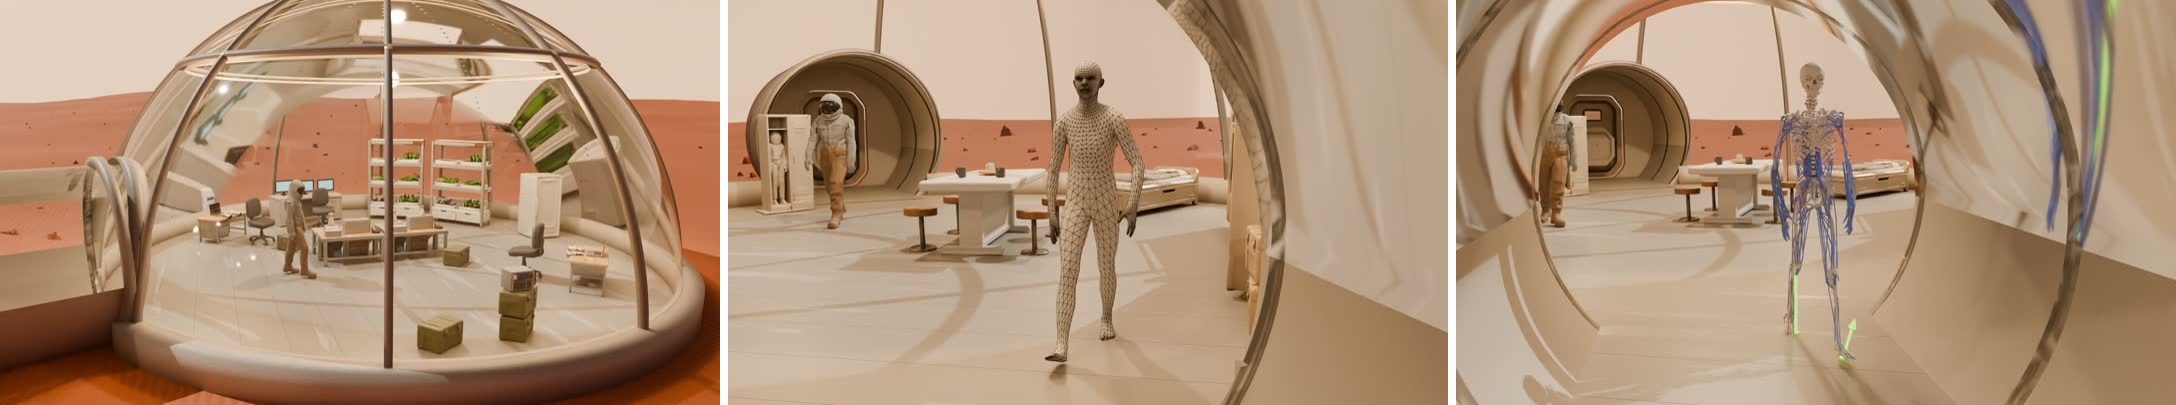
\includegraphics[width=1\linewidth,height=\textheight,keepaspectratio,alt={The peel at the end of the camp film: the player model (left), its SOMA body (centre) and its MyoFullBody sim body with its muscles and a ground reaction force arrow under the standing foot (right), walking through the tunnel between the two domes.}]{figures/peel.jpg}
\caption{The peel at the end of the camp film: the player model (left), its SOMA body (centre) and its MyoFullBody sim body with its muscles and a ground reaction force arrow under the standing foot (right), walking through the tunnel between the two domes.}
\end{figure}
